\section{Funktionenfolgen und deren Konvergenz}
\subsection{Funktionenfolgen und deren Konvergenz}
Ist $ \Omega \subset \R  $ nichtleer und für jedes $ n \in \N  $ eine Funktion $ f_n : \Omega \to \R  $ definiert, so nennen wir $ (f_n) $ eine Funktionenfolge

\begin{subexample}
	Sei für $ n \in \N \quad f_n : \Omega \to \R , x \mapsto x^n $. z.B.
	\begin{enumerate}[label=\arabic*.]
		\item $ f_1: \Omega \to \R , x \mapsto x $ 
		\item $ f_2: \Omega \to \R , x \to x^2 $
		\item usw.
	\end{enumerate}
\end{subexample}

\begin{subdefinition}[Punktweise Konvergenz]
	Sei $ \Omega \subset \R  $ nichtleer und $ f, f_1, f_2, \dotsc: \Omega \to \R  $.\\
	Wir sagen $ (f_n) $ \textbf{konvergiert punktweise gegen} $ f $, falls $ \forall x \in R $ die Folge $ (f_n(x)) $ gegen $ f(x) $ konvergiert.\\
	Gibt es ein $ f:\Omega\to \R  $, so dass $ (f_n) $ punktweise gegen $ f $ konvergiert, so nennen wir $ (f_n) $ \textbf{punktweise konvergent}.\\
	Wir nennen dann $ f $ \textbf{Grenzfunktion} von $ (f_n) $.\\
	Das bedeutet:
	\[
		\forall x \in \Omega: \forall \varepsilon > 0 : \exists N \in \N : \forall n \geq N: |f_n(x) - f(x) | < \varepsilon 
	\]
\end{subdefinition}

\begin{subexample}
	Sei $ \Omega = [0, 1] $. Wir betrachten $ f_n: \Omega \to \R  $ mit $ f_n(x) = x^n, x \in [0, 1] $.\\
	Ist $ x \in [0, 1) $, so $ \lim_{n \to \infty} f_n(x) = 0 $. Hingegen $ \lim_{n \to \infty} f_n(x) = 1 $ für $ x = 1 $.
	Also konvergiert $ (f_n) $ punktweise gegen
	\[
		f: \Omega \to \R \text{ mit } f(x) \coloneqq \begin{cases}
			0 & \text{für } 0\leq x<1\\
			1 & \text{für } x = 1
		\end{cases}
	\]
\end{subexample}
\begin{figure}[!ht]
	\centering
	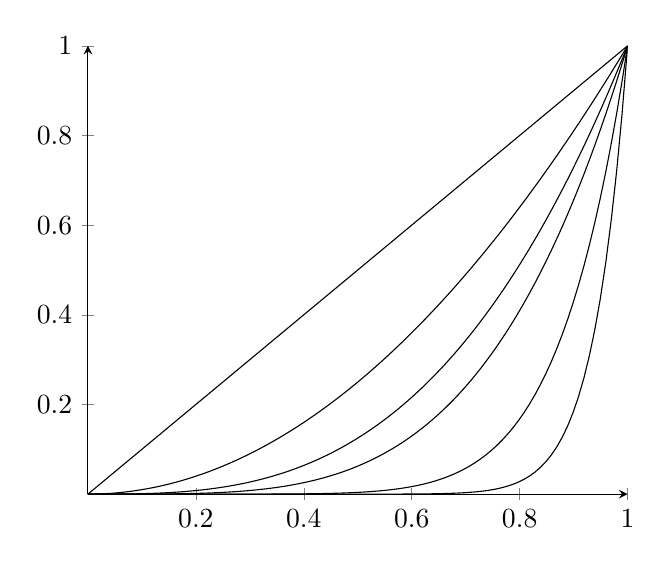
\begin{tikzpicture}
		\begin{axis}[
			xmin= 0, xmax= 1,
			ymin= 0, ymax = 1,
			axis lines = middle,
		]
			\addplot[domain=0:1, samples=100]{x};
			\addplot[domain=0:1, samples=100]{x^2};
			\addplot[domain=0:1, samples=100]{x^3};
			\addplot[domain=0:1, samples=100]{x^4};
			\addplot[domain=0:1, samples=100]{x^8};
			\addplot[domain=0:1, samples=100]{x^16};
		\end{axis}
	\end{tikzpicture}
	\begin{tikzpicture}
		\begin{axis}[
			xmin= 0, xmax= 1,
			ymin= 0, ymax = 1,
			axis lines = middle,
		]
			\addplot[domain=0:1, samples=100, color = blue]{0};
			\addplot[color = blue, mark = *, only marks] coordinates{(1,1)};
			\draw[dotted, color = blue] (axis cs:1,0) --(axis cs:1,1);
		\end{axis}
	\end{tikzpicture}
	\caption{Definition 8.1.2}
	\label{Definition8.1.2}
\end{figure}

\begin{subdefinition}
	Sei $ \Omega \subset \R  $ nichtleer und $ f, f_1, f_2, \dotsc : \Omega \to \R  $.
	Wir sagen $ (f_n) $ {\color{yellow} konvergiert gleichmäßig gegen} f, falls für jedes $ \varepsilon > 0 $ ein $ N \in \N  $ existiert, sodass $ |f(x) - f_n(x)| < \varepsilon  $ f.a. $ x \in \Omega $ und alle $ n \geq N $ gilt.\\
	Das bedeutet:
	\[
		\forall \varepsilon > 0: \exists N \in \N \forall n \geq N : \forall x \in \Omega: |f_n(x) - f(x)| < \varepsilon .
	\]
\end{subdefinition}

\begin{sublemma}
	Sei $ \Omega \subset \R  $ nichtleer und $ f, f_1, f_2, \dotsc : \Omega \to \R  $ so, dass $ (f_n) $ gleichmäßig gegen $ f $ konvergiert.
	Dann konvergiert $ (f_n) $ auch punktweise gegen $ f $.
\end{sublemma}

\begin{subexample}
	Die Folge aus Beispiel \ref{8.1.3} konvergiert nicht gleichmäßig.\\
	Sei $ 1 > \varepsilon > 0, N \in \N  $ beliebig. Setzte $ x \coloneqq \sqrt[n]{\varepsilon }   $. Dann ist $ x_0 \in (0, 1) $ und $ f_n(x_0) = \varepsilon  $, d.h. $ |f_n(x_0) - f(x_0)| = |f_n(x_0)| = \varepsilon \geq \varepsilon  $
\end{subexample}

\begin{subtheorem}
	Sei $ \Omega \subset \R  $ nichtleer und $ f_1, f_2, \dotsc : \Omega \to \R  $ stetige Funktionen.
	Konvergiert $ (f_n) $ gleichmäßig gegen $ f: \Omega \to \R  $, so ist $ f $ stetig.
\end{subtheorem}

\begin{subproof*}[Theorem \ref{8.1.7}]
	Sei $ x_0 \in \Omega $ und $ \varepsilon > 0 $ beliebeig. Dann finden wir wegen glm. Konv. ein $ N \in \N $
	mit $ |f_n(x) - f(x)| < \frac{ \varepsilon  }{ 2 }  $ ...
\end{subproof*}

$ (f_n), f_n : \Omega \to \R  $ Funktion.\\
können wir Konzepte der Folgen auch auf Funktionenfolgen anwenden?\\
$ (a_n) \subset \R \mapsto (f_n : \Omega \ni x \mapsto a_n) $
$ f, f_1, f_2, \dotsc : \Omega \to \R , f_n \to  f  $ punktweise Konvergent $ \iff \forall x \in \Omega : f(x) = \lim_{n \to \infty} f_n(x) $\\
Sind alle $ f_n $'s stetig, so nicht unbedingt $ f $!\\
\textbf{Verschärfung:} $ f_n \to f $ \textbf{gleichmäßig}, falls $ \forall \varepsilon > 0 : \exists N \in \N : \forall n \geq N : \forall x \in \Omega : | f_n(x) - f(x) | < \varepsilon  $.
\begingroup
\color{green}
\textbf{Punktweise Konvergenz}:
$ \forall x \in \Omega : \forall \varepsilon > 0 : \exists N \in \N  : \forall n \geq N : | f_n(x) - f(x) | \varepsilon  $ 
\endgroup

\begin{itemize}
	\item Bei gleichmäßiger Konvergenz $ f_n \to f: $ Alle $ f_n $'s stetig $ \implies f $ stetig.
\end{itemize}

\subsection{Normierte Vektorräume stetiger Funktionen}
\textbf{In Vektorräumen:}
\begin{itemize}
	\item Addition möglich
	\item Multiplikation mit Skalaren möglich
	\item Nullvektor ($ \hat{=} $ neutrales Element der Addition)
\end{itemize}

$ \Omega \in \R  $ nichtleer, dann bilden die stetigen Funktionen auf $ f: \Omega \to \R  $ einen \textbf{Vektorraum} (über $ \R  $), den wir \fbox{$ C(\Omega) $} nennen. Für $ \lambda, \mu \in \R , f,g \in C(\Omega): \lambda f + \mu g : \Omega \ni x \mapsto \lambda f(x) + \mu g(x) \in \R  $.\\
Der Nullvektor ist hier die Nullfunktion, $ \mathbf{0} : \Omega \ni x \mapsto 0 \in \R  $.

\textbf{Ziel:} Ordne Funktionen eine ``Länge'' zu.
\begin{subdefinition}
	Sei $ X $ ein $ \R  $-Vektorraum. Eine Abbildung $ \left|| \cdot  \right||: \to \R _{\geq 0}  $ heißt \textbf{Norm} (Längenfunktion), falls:
	\begin{enumerate}[label=(\roman*)]
		\item $ \left|| x \right|| = 0 \iff x = 0 $.
		\item $ \forall \lambda \in \R : \forall x \in X : \left|| \lambda x \right|| = \left| \lambda \right| \left|| x \right|| $
		\item $ \forall x,y \in X: \left|| x + y \right|| \leq \left|| x \right|| + \left|| y \right|| $. (Dreiecksungleichung)
	\end{enumerate}
\end{subdefinition}

\begin{subexample}
	$ C_b(\Omega) \coloneqq  \left\{ f: \Omega \to \R : f \text{stetig und beschränkt}  \right\}  $. ($ f \text{ beschränkt } \iff \exists M \geq  0 \forall  x \in  \Omega : | f(x) | \leq M $). Dies ist auch ein Vektorraum, und es definiert $ \left|\left| f \right|\right|_{\infty, \Omega} \coloneqq \sup_{x \in \Omega} | f(x) |, f \in C_b(\Omega) $ eine \textbf{Norm darauf}.
	\begingroup
	\color{blue}
	(Auf $ C(\Omega) $ \textbf{nicht:} z.B. $ \Omega = (0, 1), f(x) \coloneqq \frac{ 1 }{ x }  $, dann $ \left|\left| f \right|\right|_{\infty, \Omega} \nless \infty ) $
	\endgroup
\end{subexample}

$ \left|\left| \cdot  \right|\right|_{\infty, \Omega} $ ``Supremumsnorm'' ( $ \widehat{=} $ Länge/Größe von Funktion)

\begin{enumerate}[label=(\roman*)]
	\item[(0)] $ \left|\left| \cdot  \right|\right|_{\infty, \Omega} : C_b(\Omega) \to  \R_{\geq 0} $. (Hier geht ein: $ f \in C_b(\Omega) $ beschränkt)
\item $ f \in C_b(\Omega) \wedge \underbrace{\left|\left| f \right|\right|}_{\infty, \Omega} = 0 $, zu zeigen \fbox{$ f = 0 $}
		\[
			\sup_{x \in \Omega} | f(x) = 0 \implies (\forall x \in  \Omega : f(x) = 0) \implies f = 0.
		\]
		und $ \left|\left| \mathbb{0} \right|\right|_{\infty, \Omega} = \sup_{x \in \Omega} 0 = 0 $.
	\item $ \lambda \in \R , f \in C_b(\Omega) $, so ist $ \forall x \in \Omega : | \lambda f(x) | =  $ 
		\begin{align*}
			~&= |lambda| |f(x)| \implies  \left|\left| \lambda f \right|\right|_{\infty, \Omega} \\
			~&= \sup_{x\in \Omega} | \lambda f (x) | \\
			~&= \sup_{x \in \Omega} |\lambda| \cdot |f(x)| \\
			~&= |\lambda| \sup_{x \in \Omega} |f(x)| \\
			~&= |\lambda| \cdot \left|\left| f \right|\right|_{\infty, \Omega}. \\
		\end{align*}
	\item $ f, g \in  C_b(\R ) $. Dann $ \forall x \in \Omega: | f(x) + g(x) | \leq \underbrace{|f(x)|}_{\leq \left|\left| f \right|\right|_{\infty, \Omega}} + \underbrace{g(x)}_{\leq \left|\left| g \right|\right|_{\infty, \Omega}} \leq \left|\left| f \right|\right|_{\infty, \Omega} + \left|\left| g \right|\right|_{\infty, \Omega} $. Supremum in $ x $
\end{enumerate}

\begin{itemize}
	\item Beachte: $ (\R , \left|\left| \cdot  \right|\right|)  $ ist auch normierter Raum.
\end{itemize}
\textbf{Konvergenz:} $ \forall \varepsilon > 0 : \exists N \in  \N  : \forall n \geq N : \left|\left| x_n - x \right|\right| < \varepsilon  $ 

\begin{subdefinition}
	Sei $ (X, \left|\left| \cdot  \right|\right| ) $ normierter Vektorraum, sowie $ x, x_1, x_2, \dotsc \in X $. Wir sagen, $ (x_n) $ \textbf{konvergiert} bezüglich $ \left|\left| \cdot  \right|\right|  $ gegen $ x $, falls $ \forall \varepsilon > 0: \exists N \in \N : \forall n \geq N : \left|\left| x_n - x  \right|\right| < \varepsilon $
\end{subdefinition}

\begin{subproposition}
	Sei $ \Omega \subset \R  $ nichtleer, $ f, f_1, \dotsc \in C_b(\Omega) $.
	Dann konvergiert $ (f_n) $ genau dann gleichmäßig gegen $ f $, wenn $ (f_n) $ bezüglich $ \left|\left| \cdot  \right|\right|_{\infty, \Omega} $ gegen $ f $ konvergiert.
	{\color{green} $ \iff \lim_{n \to \infty} \left|\left| f_n - f \right|\right|_{\infty, \Omega} = 0 $}
	\begin{description}
		\item[``$ \implies  $'']
			\begin{align*}
				&\forall \varepsilon > 0: \exists N \in \N  : \forall  n \geq  N : ( \forall x \in \Omega: |f_n(x) - f(x)| < \varepsilon )\\
				&\forall \varepsilon > 0: \exists N \in \N  : \forall  n \geq  N : \left( \sup_{x \in \Omega}: |f_n(x) - f(x)| \leq  \varepsilon \right)\\
				&(\forall \varepsilon > 0: \exists N \in \N  : \forall  n \geq  N : | |f_n(x) - f(x)| |_{\infty, \Omega} \leq  \varepsilon ) \implies  f_n \to f, \left|\left| \cdot  \right|\right|_{\infty, \Omega} \qed
			\end{align*}
	\end{description}
\end{subproposition}

\begin{subexample}
	$ f_n : \R  \ni x \mapsto \frac{ 1 }{ n(1 + x^2) } \in \R  $.\\
	\textbf{Punktweise Konvergenz} $ f_n(x) = \frac{ 1 }{ n } \cdot \left(  \frac{ 1 }{ 1 + x^2 } \right) \to 0 $.
	Also $ f_n \to 0 $ punktweise konvergent.\\
	\textbf{Gleichmäßig Konvergent} bedeutet nach Proposition \ref{8.2.4}:
	\begin{align*}
		\lim_{n \to \infty} \sup_{x \in \R } |f_n(x) - \underbrace{f(x)}_{0}| &= \left( \lim_{n \to \infty} \left|\left| f_n - f \right|\right|_{\infty, \omega} \right) \\
		~&= 0 \\
	\end{align*}
	\textbf{Hier:}
	\[
		\sup_{x \in \R } |f_n(x) - \underbrace{f(x)}_{=0} = \frac{ 1 }{ n } \underbrace{\sup_{x \in \R} \frac{ 1 }{ 1+x^2 }  }_{=1} = \frac{ 1 }{ n } ,
	\]
	also 
	\[
		\lim_{n \to \infty} \left|\left| f_n - f \right|\right|_{\infty, \Omega} = \lim_{n \to \infty} \frac{ 1 }{ n } = 0.
	\]
	gleichmäßige Konvergenz
\end{subexample}

\begin{subexample}
	\[
		f_n : [0, 1] \ni x \mapsto x^n \in \R,
	\]
	so $ f_n \to f $ punktweise konvergent mit
	\[
		f(x) = \begin{cases}
			0, & x \in [0, 1),\\
			1, & x = 1
		\end{cases}.
	\]
	Haben 
	\[
		\sup_{x \in [0, 1]} | f_n(x) - f(x)| = \sup_{x \in [0, 1)} | x^n | \overset{n\to \infty}{\nrightarrow} 0
	\]
	
\end{subexample}

